% !TEX root = ../CourseOT.tex

%%%%%%%%%%%%%%%%%%%%%%%%%%%%%%%%%%%%%%%%%%%%%%%%%%%%%%%%%%%%%%%%%%%%%%%%%%%
%%%%%%%%%%%%%%%%%%%%%%%%%%%%%%%%%%%%%%%%%%%%%%%%%%%%%%%%%%%%%%%%%%%%%%%%%%%
%%%%%%%%%%%%%%%%%%%%%%%%%%%%%%%%%%%%%%%%%%%%%%%%%%%%%%%%%%%%%%%%%%%%%%%%%%%
\section{Optimal Matching between Point Clouds}

%%%%%%%%%%%%%%%%%%%%%%%%%%%%%%%%%%%%%%%%%%%%%%%%%%%%%%%%%%%%%%%%%%%%%%%%%%%
\subsection{Monge Problem between Discrete points}

%%%%%%%
\paragraph{Matching problem}

Given a cost matrix $(\C_{i,j})_{i \in \range{n}, j \in \range{m}}$, assuming $n=m$, the optimal assignment problem seeks for a bijection $\si$ in the set $\Perm(n)$ of permutations of $n$ elements solving
\eql{\label{eq-optimal-assignment}
	\umin{\si \in \Perm(n)} \frac{1}{n}\sum_{i=1}^n \C_{i,\si(i)}.
}
One could naively evaluate the cost function above using all permutations in the set $\Perm(n)$. However, that set has size $n!$, which is gigantic even for small $n$. Consider for instance that such a set has more than $10^{100}$ elements~\cite{Dantzig1983} when $n$ is as small as 70. That problem can therefore only be solved if there exist efficient algorithms to optimize that cost function over the set of permutations, which will be the subject of~\S\ref{s-matching}.

\begin{rem}[Uniqueness] Note that the optimal assignment problem may have several optimal solutions. Suppose for instance that $n=m=2$ and that the matrix $\C$ is the pairwise distance matrix between the 4 corners of a 2-dimensional square of side length $1$, as represented in the left plot in Figure~\ref{fig-non-unique-matching}. In that case only two assignments exist, and they share the same cost.
\end{rem}

\begin{figure}
\centering
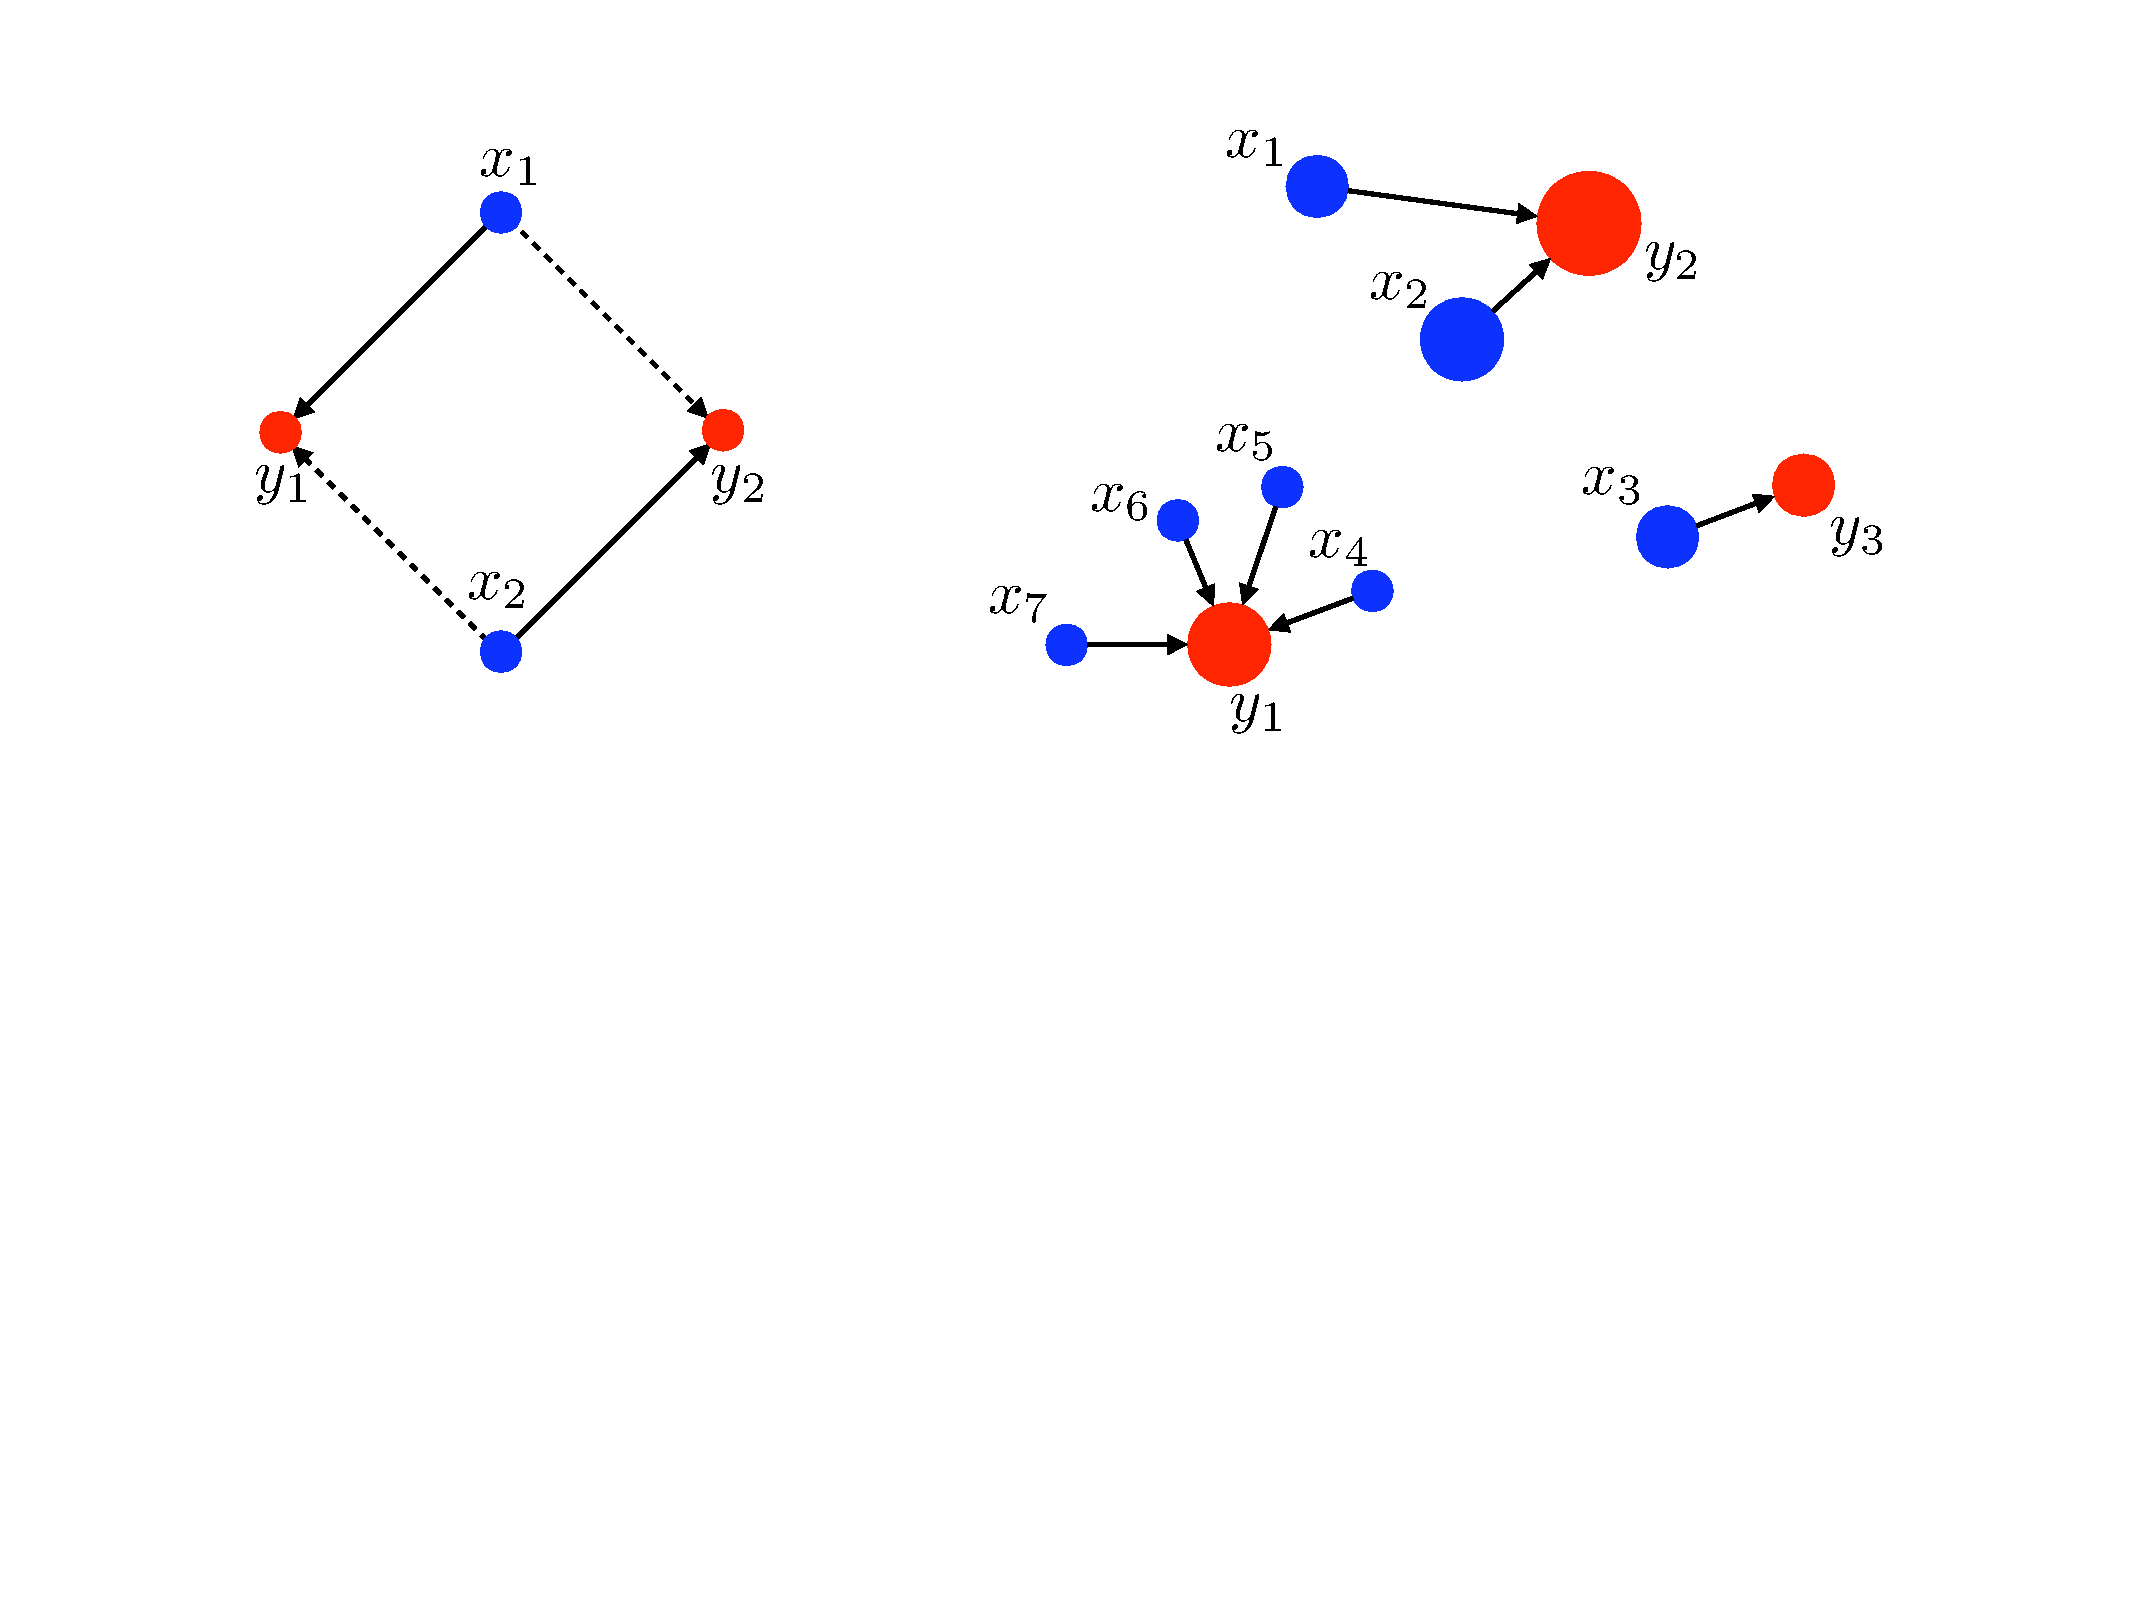
\includegraphics[width=.5\linewidth]{non-unique-optimal-matching/non-unique-optimal-matching}
\caption{\label{fig-non-unique-matching}
(left) blue dots from measure $\alpha$ and red dots from measure $\beta$ are pairwise equidistant. Hence, either matching $\sigma=(1,2)$ (full line) or $\sigma=(2,1)$ (dotted line) is optimal. (right) a Monge map can associate the blue measure $\alpha$ to the red measure $\beta$. The weights $\alpha_i$ are displayed proportionally to the area of the disk marked at each location. The mapping here is such that $T(x_1)=T(x_2)=y_2$, $T(x_3)=y_3$, whereas for $4\leq i\leq 7$ we have $T(x_i)=y_1$.
}
\end{figure}


\paragraph{1D case}

Here $\X=\RR$. Assuming $\al = \frac{1}{n}\sum_{i=1}^n \de_{x_i}$ and $\be = \frac{1}{n}\sum_{j=1}^n \de_{y_j}$, and assuming (without loss of generality) that the points are ordered, \emph{i.e.} $x_1 \leq x_2 \leq \ldots \leq x_n$ and $y_1 \leq y_2 \leq \ldots \leq y_n$, then one has the simple formula
\eql{\label{eq-1d-empirical}
	\Wass_p(\al,\be)^p = \sum_{i=1}^p |x_i-y_i|^p, 
}
\emph{i.e.} locally (if one assumes distinct points), $\Wass_p(\al,\be)$ is the $\ell^p$ norm between two vectors of ordered values of $\al$ and $\be$. That statement is only valid locally, in the sense that the order (and those vector representations) might change whenever some of the values change. That formula is a simple consequence of the more general remark given below. 
%
Figure~\ref{fig-1d-discrete}, top row, illustrates the 1-D transportation map between empirical measures with the same number of points. 
 The bottom row shows how this monotone map generalizes to arbitrary discrete measures. 
%
It is possible to leverage this 1-D computation to also compute efficiently OT on the circle, see~\cite{delon-circle}.  
%
Note that in the case of concave cost of the distance, for instance when $p<1$, the behaviour of the optimal transport plan is very different, see~\cite{delon-concave}, which describes an efficient solver in this case.



\begin{figure}
\centering
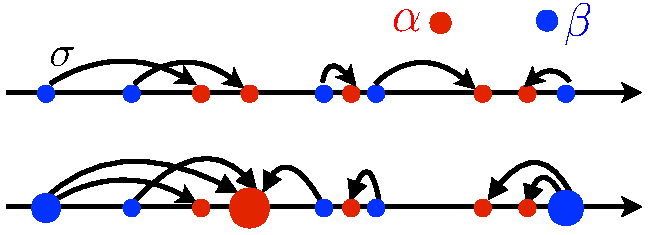
\includegraphics[width=.4\linewidth]{1d-discrete/1d-schematic}
\caption{\label{fig-1d-discrete}
1-D optimal couplings: each arrow $x_i \rightarrow y_j$ indicate a non-zero $\P_{i,j}$ in the optimal coupling.
% 
Top: empirical measures with same number of points (optimal matching).
Bottom: generic case. 
%
This corresponds to monotone rearrangements, if $x_i \leq x_{i'}$ are such that $\P_{i,j} \neq 0, \P_{i',j'} \neq 0$, then necessarily $y_j \leq y_{j'}$.
}
\end{figure}


- application to  Gray scale equalization, code via sorting , nlogn

%%%%%%%%%%%%%%%%%%%%%%%%%%%%%%%%%%%%%%%%%%%%%%%%%%%%%%%%%%%%%%%%%%%%%%%%%%%
\subsection{Matching Algorithms}

- Algorihtm : hungarian (explain intuitively) / auction (see later)
  Appli 3D color equalization